% !TEX root = thesis.tex
\documentclass[
11pt,
a4paper,
abstracton,
numbers=noenddot,
listof=totoc,
bibliography=totoc,
twoside,
openright,
cleardoublepage=plain,
parskip=half+, % comment this out if you do not want an empty half line between paragraphs, but please read the KomaScript Guide and search for parskip (around page 82): ftp://ftp.dante.de/pub/tex/macros/latex/contrib/koma-script/scrguide.pdf
BCOR=1cm, % Bindekorrektur: Change this accordingly, also read the KomaScript Guide! Make sure you read the guide.
]{scrreprt}

% % % % % % % % % % % % % % % % % % % % % % % % % % % % % % % % %
% EDIT THE DATA IN THIS BLOCK TO YOUR INFORMATION				%
% % % % % % % % % % % % % % % % % % % % % % % % % % % % % % % % %
% Set data about yourself										%
\newcommand{\authorname}{Jan Philipp Berg, Simon Keil}								%
\newcommand{\studentnumber}{000000, 000000}	% Matrikelnummer			%
\newcommand{\courseofstudy}{Information Systems} % Studiengang	%
																%
% Set data about your thesis									%
\newcommand{\thesistitle}{Implementation of the Advanced Encryption Standard}		%
\day=07 \month=12 \year=2020									%
																%
% Set thesis type and language									%
\newcommand{\thtype}{Seminar}	% Bachelor, Master or Seminar	%
\newcommand{\thesislanguage}{English}	% English or German		%
% % % % % % % % % % % % % % % % % % % % % % % % % % % % % % % % %

% if you really need additionall packages include them here
%\usepackage{package}
\usepackage{tcolorbox}

% DO NOT EDIT THE _settins FILE!
% General stuff
\usepackage{fixltx2e}
\usepackage[utf8]{inputenc} % CHANGE HERE IF NECESSARY
\usepackage[T1]{fontenc}
\usepackage[english]{babel} % last language given is used (here: english) #ngerman,
%\usepackage{microtype}
\usepackage{ifpdf}
\usepackage{verbatim}
\usepackage{float}

\author{\authorname}
\title{\thesistitle}
\date{\today}

% Figures
\usepackage{graphicx}
\usepackage{subfig}
\usepackage{placeins}

% Tables
\usepackage{booktabs}
\usepackage{marvosym}
\usepackage{multirow}

% Math stuff and units
\usepackage{latexsym,amsmath, amssymb, amsfonts, upgreek}
\usepackage{siunitx}
\newcommand{\mathup}{\mathrm}

% Acronyms
\usepackage[printonlyused]{acronym}

% Enable quotes by \enquote{}
\usepackage[babel,english=american]{csquotes}

% Necessary for frontpage, allows to create automata and fancy graphics
\usepackage{tikz}

% Protocols and bytefields
\usepackage{protocol}
\usepackage{bytefield}

% Source code listings
\definecolor{colKeys}{rgb}{0,0,1}
\definecolor{colIdentifier}{rgb}{0,0,0}
\definecolor{colComments}{rgb}{1,0,0}
\definecolor{colString}{rgb}{0,0.5,0}

\usepackage{listings}
\lstset{%
	float=hbp,%
	basicstyle=\ttfamily\scriptsize, %
	identifierstyle=\color{colIdentifier}, %
	keywordstyle=\color{colKeys}, %
	stringstyle=\color{colString}, %
	commentstyle=\color{colComments}, %
	columns=flexible, %
	tabsize=2, %
	frame=single, %
	extendedchars=true, %
	showspaces=false, %
	showstringspaces=false, %
	numberstyle=\tiny, %
	breaklines=true, %
	backgroundcolor=, %
	breakautoindent=true, %
	captionpos=b%
}

% Algorithms
\usepackage[ruled, vlined, linesnumbered, algosection, algo2e]{algorithm2e}

% Format page foot and header
\usepackage{scrlayer-scrpage}
\clearscrheadings
\clearscrheadfoot
\automark[section]{chapter}
\ohead{\pagemark}
\ihead{\headmark}
\pagestyle{scrheadings}

%% use some standards for mathematical expressions:
\newcommand{\red}{{\rm red}}
\newtheorem{theorem}{Theorem}[section]
\newtheorem{lemma}[theorem]{Lemma}
\newtheorem{proposition}[theorem]{Proposition}
\newtheorem{corollary}[theorem]{Corollary}
% \newtheorem{definition}[theorem]{Definition}
\newtheorem{algorithm}[theorem]{Algorithm}
\newenvironment{example}{\begin{quote}{\bf Example:}}{\end{quote}}

% Bibliography
\bibliographystyle{alpha}

% gray definition boxes, that whay you'll find them in the text
\usepackage{shadethm}
\newshadetheorem{sthm}{Definition}[chapter]
\newenvironment{definition}[1][]{
	\definecolor{shadethmcolor}{rgb}{.9,.9,.9}
	\begin{sthm}[#1]
	}{\end{sthm}}

% experimental
%\usepackage{scrhack}
\usepackage{paralist}
% Hyperlinks and menu for your document
\usepackage[breaklinks,hyperindex,colorlinks,anchorcolor=black,citecolor=black,filecolor=black,linkcolor=black,menucolor=black,urlcolor=black,pdftex]{hyperref}

% pagebackref: Add page number to the references where they can be found
% DO NOT LOAD ANY OF YOUR PACKAGES BEYOND THIS PACKAGE

\makeatletter
\AtBeginDocument{
	\hypersetup{
		pdftitle = {\@title},
		pdfauthor = {\@author},
		pdfsubject={\@title},
		pdfkeywords={Template, LaTeX, SysSec, Sensor fingerprinting, Accelerometer, Smartphone, Mobile Device}, % CHANGE HERE
		%    unicode={true},
	}
}
\makeatother

% \ifpdf
% 	\hypersetup{linktocpage=false} 	% false=links are section names, true=links are page numbers, IMPORTANT: in dvi2ps mode, 'true' is required!
% \else
% 	\hypersetup{linktocpage=true} 		% false=links are section names, true=links are page numbers, IMPORTANT: in dvi2ps mode, 'true' is required!
%  \usepackage[hyphenbreaks]{breakurl}
% \fi

\newcommand{\declarationofauthorship}[2]{%
	\ifthenelse{\equal{#1}{German}}
	{\chapter*{Eidesstattliche Erklärung}
	Ich versichere hiermit, dass ich diese \thtype-Arbeit mit dem Titel \glqq{#2}\grqq
	selb\-st\"{a}n\-dig und ohne fremde Hilfe angefertigt habe, und dass ich alle von anderen Autoren w\"{o}rtlich \"{u}\-ber\-nom\-men\-en Stellen wie auch die sich an die Ge\-dan\-ken\-g\"{a}n\-ge anderer Autoren eng anlehnenden Aus\-f\"{u}h\-run\-gen meiner Arbeit besonders
	gekennzeichnet und die Quellen zitiert habe.

	\vspace{2cm}
	\rule{4cm}{0.1pt} \hfill \rule{7cm}{0.1pt} \\
	\hspace*{1.75cm} \textsc{Datum} \hspace*{6.8cm} \textsc{Unterschrift}
	}
	{\chapter*{Declaration}
		I hereby declare that, to the best of my knowledge and belief, this \thtype thesis titled ``{#2}'' is my own work. I confirm that each significant contribution to and quotation in this thesis that originates from the work or works of others is indicated by proper use of citation and references.

	\vspace{2cm}
	\rule{4cm}{0.1pt} \hfill \rule{7cm}{0.1pt} \\
	\hspace*{1.75cm} \textsc{Date} \hspace*{6.8cm} \textsc{Signature}
	}
}


\newcommand{\consentforplagiarismdetection}[5]{%
	\ifthenelse{\equal{#1}{German}}
	{\chapter*{Einverständniserklärung}
		{\small
		zur Prüfung meiner Arbeit mit einer Software zur Erkennung von Plagiaten

		\begingroup
			\textbf{Name}:~{#2}\newline
			\textbf{Matrikelnummer}:~{#3}\newline
			\textbf{Studiengang}:~{#4}\newline
			\textbf{Titel der Arbeit}:~{#5}\newline
		\endgroup

		\textbf{Was ist ein Plagiat?}
		Als ein Plagiat wird eine Übernahme fremden Gedankengutes in die eigene Arbeit angesehen, bei der die Quelle, aus der die Übernahme erfolgt, nicht kenntlich gemacht wird. Es ist dabei unerheblich, ob z.B. fremde Texte wörtlich übernommen werden, nur Strukturen (z.B. argumentative Figuren oder Gliederungen) aus fremden Quellen entlehnt oder Texte aus einer Fremdsprache übersetzt werden.

		\textbf{Softwarebasierte Überprüfung}
		Alle Bachelor- und Masterarbeiten werden vom Prüfungsamt mit Hilfe einer entsprechenden Software auf Plagiate geprüft. Die Arbeit wird zum Zweck der Plagiatsüberprüfung an einen Software-Dienstleister übermittelt und dort auf Übereinstimmung mit anderen Quellen geprüft. Zum Zweck eines zukünftigen Abgleichs mit anderen Arbeiten wird die Arbeit dauerhaft in einer Datenbank gespeichert. Ein Abruf der Arbeit ist ausschließlich durch die Wirtschaftswissenschaftliche Fakultät der Westfälischen Wilhelms-Universität Münster möglich. Der Studierende erklärt sich damit einverstanden, dass allein zum beschriebenen Zweck der Plagiatsprüfung die Arbeit dauerhaft gespeichert und vervielfältigt werden darf. Das Ergebnis der elektronischen Plagiatsprüfung wird dem Erstgutachter mitgeteilt.

		\textbf{Sanktionen}
		Liegt ein Plagiat vor, ist dies ein Täuschungsversuch i.S. der Prüfungsordnung, durch den die Prüfungsleistung als \enquote{nicht bestanden} gewertet wird. Es erfolgt eine Mitteilung an das Prüfungsamt und die dortige Dokumentation. In schwerwiegenden Täuschungsfällen kann der Prüfling von der Prüfung insgesamt ausgeschlossen werden. Dies kann unter Umständen die Exmatrikulation bedeuten. Plagiate können auch nach Abschluss des Prüfungsverfahrens und Verleihung des Hochschulgrades zum Entzug des erworbenen Grades führen.


		Hiermit erkläre ich, dass ich die obigen Ausführungen gelesen habe und mit dem Verfahren zur Aufdeckung und Sanktionierung von Plagiaten einverstanden bin.
		}

		\vspace{2cm}
		\rule{4cm}{0.1pt} \hfill \rule{7cm}{0.1pt} \\
		\hspace*{1.75cm} \textsc{Datum} \hspace*{6.8cm} \textsc{Unterschrift}
	}
	{\chapter*{Consent Form}
	{\small
		for the use of plagiarism detection software to check my thesis

		\begingroup
		\textbf{Full Name}:~{#2}\newline
		\textbf{Student Number}:~{#3}\newline
		\textbf{Course of Study}:~{#4}\newline
		\textbf{Title of Thesis}:~{#5}\newline
		\endgroup

		\textbf{What is plagiarism?}
		Plagiarism is defined as submitting someone else's work or ideas as your own without a complete indication of the source. It is hereby irrelevant whether the work of others is copied word by word without acknowledgment of the source, text structures (e.g. line of argumentation or outline) are borrowed or texts are translated from a foreign language.

		\textbf{Use of plagiarism detection software}
		The examination office uses plagiarism software to check each submitted bachelor and master thesis for plagiarism. For that purpose the thesis is electronically forwarded to a software service provider where the software checks for potential matches between the submitted work and work from other sources. For future comparisons with other theses, your thesis will be permanently stored in a database. Only the School of Business and Economics of the University of Münster is allowed to access your stored thesis. The student agrees that his or her thesis may be stored and reproduced only for the purpose of plagiarism assessment. The first examiner of the thesis will be advised on the outcome of the plagiarism assessment.

		\textbf{Sanctions}
		Each case of plagiarism constitutes an attempt to deceive in terms of the examination regulations and will lead to the thesis being graded as \enquote{failed}. This will be communicated to the examination office where your case will be documented. In the event of a serious case of deception the examinee can be generally excluded from any further examination. This can lead to the exmatriculation of the student. Even after completion of the examination procedure and graduation from university, plagiarism can result in a withdrawal of the awarded academic degree.

		I confirm that I have read and understood the information in this document. I agree to the outlined procedure for plagiarism assessment and potential sanctioning.
		}

		\vspace{2cm}
		\rule{4cm}{0.1pt} \hfill \rule{7cm}{0.1pt} \\
		\hspace*{1.75cm} \textsc{Date} \hspace*{6.8cm} \textsc{Signature}
	}
}


% your document starts here
\begin{document}

% title page - no need to edit
% !TEX root = thesis.tex
\begin{titlepage}
\makeatletter

\enlargethispage{3cm}

\begin{minipage}{0.45\textwidth}
	
\includegraphics[width=\textwidth]{data/assets/wwu-logo}
\end{minipage}
%\hfill
\hspace{.1\textwidth}
\begin{minipage}{0.45\textwidth}
	
\includegraphics[width=\textwidth]{data/assets/faculty-de}
\end{minipage}


\vspace*{10cm}
\begin{minipage}[b]{1\linewidth}
	\sffamily
  	\hspace{-17.2mm}
  	% \includegraphics[scale=1.0]{data/logo/rub_slogan}\\

   	\textbf{\LARGE {\@title}}\\

  	\Large{\@author}\\

% 	\vspace*{35mm}
	\vspace{4cm}
  	\normalsize{
   	\thtype\/ Thesis\@~~--~~\@date\@.\\
   	Cyber Security\\Department of Information Systems\\
   	University Münster, Germany\\}
	\newline
	\normalsize{
	\begin{tabular}{@{}ll@{}}
	Principal Supervisor: Prof.~Dr.-Ing.~Thomas~Hupperich\\
%	Associate Supervisor: XXXXXXXXXX\\
	%Advisor: & Another Guy, Maybe Another\\
	\end{tabular}
	}
\end{minipage}


\makeatother
\end{titlepage}


% give a short abstract of your thesis
%\begin{abstract}
The usage of smartphones has become quite popular in the last decade. Every new smartphone model contains new hardware features, thus making people more attracted to benefit from these features. But the more features a smartphone contains, the more potential privacy and security issues arise from these features. Many of these features utilize the various built-in smartphone sensors like the accelerometer. Accelerometer data lead to the ability for installed applications to track the user's actual condition and activity. Previous laboratory studies have proved that hardware imperfections during the accelerometer manufacturing process, provide the possibility to recognize smartphones by utilizing signal feature extraction. In our approach, we demonstrate whether this method is applicable to recognize device models just as well as unique devices.
\end{abstract}
\clearpage

\cleardoublepage
\pagestyle{scrheadings} % reenable headers and footers
\tableofcontents

% include all your chapters as .tex files,
% each file contains sections \section{name of section},
% subsections \subsections{...} and so on...

\chapter{Introduction} \label{chap:intro}
%\pagenumbering{arabic} %switches to arabic numbers for the rest of the text
% !TEX root = thesis.tex
% Always start a chapter with a short but informative text about the following sections\@. Point out the relevance of the sections and create interconnections between them\@. Never ever just write a single sentence here\@. Furthermore,\ you are strongly advised to respect the hints given in this template\@.

In this chapter, we will give an overview on our motivation and the setting of the implementation of the Advanced Encryption Standard, followed by an outline of the structure of this thesis.
 

\section{Motivation}
\label{ch:motivation}
The more our lives shift into the internet the more important becomes protection of it and the data it represents, not least, because of the ever increasing dangers lurking in the world wide web. This protection can partially be archieved through encryption, which is why it and with that the Advanced Encryption Standard is found nearly everywhere in the digital realm. The majority  of instant messengers used \cite{instantmessages} are encrypted with the Signal protocol\cite{whatsapp}\cite{fbmessenger}\, which uses \ac{AES} at its heart \cite[ch. 5.2]{signal}. Windows only enables TLS with \ac{AES} as a default \cite{wintls} and nearly 85\% of webpages loaded via Firefox use https and thus TLS \cite{fftelem}. Android \cite{android} and iOS \cite{ios}encrypt all devices by default with \ac{AES}. 

But how does this encryption algorithm work and why does it seem to enjoy such widespread trust? The following document gathers some information on \ac{AES} and outlines the implementation process of the algorithm.

\section{Setting}
\label{ch:setting}

This document provides detailed information over the algorithm itself and the planning process involved in an implementation of \ac{AES}, showing which parts were done by which team member and demonstrating project management ability. It is part of the project seminar "Implementing the Advanced Encryption Standard" and will be supplemented by an actual implementation and the documentation of this implementation.

\section{Organization of this Thesis}
\label{ch:organizationofthisthesis}

The second chapter adresses the background of \ac{AES}. First a quick overview on the developements of digital encryption is given and what \ac{AES} means in that context. Then the selection process of \ac{AES} is discussed. Finally some reactions of the cryptographic community to \ac{AES} are gathered and summarized.
The third chapter describes in detail, how the project was planned. It walks through the different phases of project developement and applies each phase to the present project, giving insights in how the final result was realized.


\chapter{Background} \label{chap:background}
% !TEX root = thesis.tex
This chapters purpose is to give context to the AES algorithm. It starts with a brief history of cryptography, explains the AES-selection-process and then gives some examples of security issues that have been found over the years.


\section{Before AES}
\label{ch:before-aes}
Cryptography or the art of concealing meaning in writing ist over 4000 years old.

The advent of the electronic computer changed the field of cryptography fundamentally. Starting with the "bombe", produced by Alan Turing and refined by Gordon Welchman around 1940, the world ushered into a new era of automated de- and encryption. 
The bombe is an electro-mechanical device that was key to breaking the ciphers produced by the enigma - a device used by the german military in the second world war to secure their communications. Turings bombe was the first machine that was able to break message encryption in an automated fashion. Previously cryptoanalysts had to break ciphers "by hand" i.e. by doing manual frequency analysis for example. Breaking the enemies communication provided a vital advantage for the Allies during World War Two.
The next cryptographic revolution came in 1971 when Whitfield Diffie invented public-key-cryptography, single-handedly eliminating a problem that haunted cryptographers from the beginnigs of their field of expertise: the establishing of a shared secret over insecure channels, also known as the key distribution problem. Previously the security of an encryption scheme based on the fact, that there was atleast one element in said scheme, that must remain unknown to malicious parties intending to attack and decipher the communication, for example a password. Public-key-cryptography does not work like this: Parties wishing to communicate simply exchange their public keys over an unsecured channel and are able to establish a guaranteed shared secret from that. Without knowing the corresponding private keys, the public keys are worthless in the eyes of an attacker. But the maths behind Public-key-cryptography is prohibitively expensive if one attemts to encrypt something this way by hand. Progress like this was only possible by utilising electronic computers.
When those computers later on became widely available for a broader range of people, suddenly everyone was able to encrypt information with complicated schemes. And for the first time the security of those schemes was mathematically provable. In fact the prove of some of those later schemes guaranteed protection even from entities with massive resources, manpower and expertise without the need for skilled and qualified cryptographers. 
The first openly available standart for electronic encryption was a symmetric cipher called "Data Encryption Standard" or DES. Developed in the early 1970s at IBM the cipher was published in 1977 as an official Federeal Information Processing Standard (FIPS). The security of DES was disputed right from its first publication. Even in the late seventies the key length was critisized as too short, although it took until June of 1997 before the first DES message was publicly decrypted via brute force attack. In January of the same year the search for a predecessor of DES was announced by the National Institute of Standards and Technology of the United States (NIST). This predecessor supposed to be "an unclassified, publicly disclosed encryption algorithm capable of protecting sensitive government information well into the next century." To increase trust into this standard-to-be the search was public and NIST relied on submissions from the cryptographic community. 


\section{The Advanced Encryption Standart selection}
\label{ch:aes-selection}

The following chapter is, if not mentioned otherwise, based on \cite{nistdevoverview}.

The formal call for submissions of AES canidates came in september of 1997. NIST explicitly requested input from outside of the institution by explicitly asking "the public, academic/research communities, manufacturers, voluntary standards organizations, and Federal, state, and local government organizations." The submissions would be made public for review and comment after the submission period

\subsection{Requirements}
\label{ch:requirements}

The proposed algorithms for the new encrytion standard and thus the
potential successors of DES had to fullfill a number of requirements, as can be found in \cite{announcementrequest}, in order for them to be concidered by NIST. AES was intended to be a block
cipher operating on 128 bits at a time. Those bits should be secured by
key length of atleast the three sizes 128, 192 and 256 bits. 
The canidates would be furthermore analyzed and evaluated regarding:

\begin{itemize}
\item
  \emph{security}: Deemed as the most important criterion, it
  encompasses factors like the actual security compared to the
  competitors, the degree to which the algorithm is able to produce an
  output indistinguishable to a random permutation of the input, the
  quality of the mathematical prinicples behind the algorithm and of
  course critique, concerns and attacks regarding the canidate
  originating from the public review.
\item
  \emph{cost}: Financial cost was one concideration: All canidates had
  to be released on a ``worldwide, non-exclusive, royalty-free basis.''
  before they could be submitted. Performance costs like the speed of
  the algorithm both in software and hardware implementations or memory
  size, be it in code size, gate count for hardware implementations or
  RAM requirements for software implementations were further factors
  that played a role in this category.
\item
  \emph{algorithm and implementation characteristics}: Flexibility
  without compromising security was another desirable aspect of the new
  standard. Additonal key sizes to those specified in the minimum
  requirements, the possibility of implementation on a variety of
  platforms, from slower 8-bit SmartCard processors to fully-fledged
  desktop CPUs and other fields of applications like usage as a stream
  cipher, message authentication generator, pseudorandom number
  generator, hashing algorithm and more were all attributes to the
  flexibility of an encryption algorithm an thus factors, that
  influenced the AES-comittee in their final decision. The last aspect
  under which the standard-to-be had to prove itself was simplicity,
  where a simpler algorithm, that holds up well under all other aspects,
  is preferable.
\end{itemize}


\subsection{The AES selection process}
\label{ch:aes}


Nearly a year after requesting submissions, NIST published a list with fifteen canidates they deemed worthy of further investigation at the First AES Canidate Conference (AES1) in August 1998. The cryptographic community was invited to critique those choices, either via email or later on in the online discussion forum NIST hosted for this exact purpose. This input from the community collected in "Round 1" of the selection process was discussed at the Second AES Canidate Conference (AES2) in spring of 1999. Shortly after that NIST selected in their publication \cite{round1report} five finalists from the initial fifteen algorithms: MARS, RC6, Rijndael, Serpent, and Twofish.
The other canidates were excluded, partially because "serious questions [had] been raised about [their] security" (p.34), partially because they were slower/potentially less secure than other comparable canidates.
The finalists moved on to recieve further scrutiny from both the NIST and the cryptographic community in the so called "Round 2".
After this more in-depth analysis of the algorithms a third conference (AES2) in April 2000 provided an open, public forum to review and discuss the findings accumulated up to this point in Round 2. The authors of the finalists were explicitly invited to partake in the process. A month later Round 2 came to an end and NIST moved on to select the algorithm they deemed to be best suited to be the Advanced Encryption Standard. 
On October of the same year the institute announced in \cite{round2report} their decision to propose Rijndael, authored by Joan Daemen and Vincent Rijmen, as the AES. Each finalist "appears  to  offer adequate security, and each offers a considerable number of advantages" (p.91), but "Rijndael’s combination of security, performance, efficiency, implementability, and flexibility make it an appropriate selection for the AES" (p.92).
The proposal was formalized in a FIPS draft for AES and published on February 2001 (\cite{fipsdraft}. After going throught the usual FIPS-approval-process the Advanced Encryption Standard was made public as FIPS 197 \cite{fips197} at the end of the year.

\begin{figure}
\centering
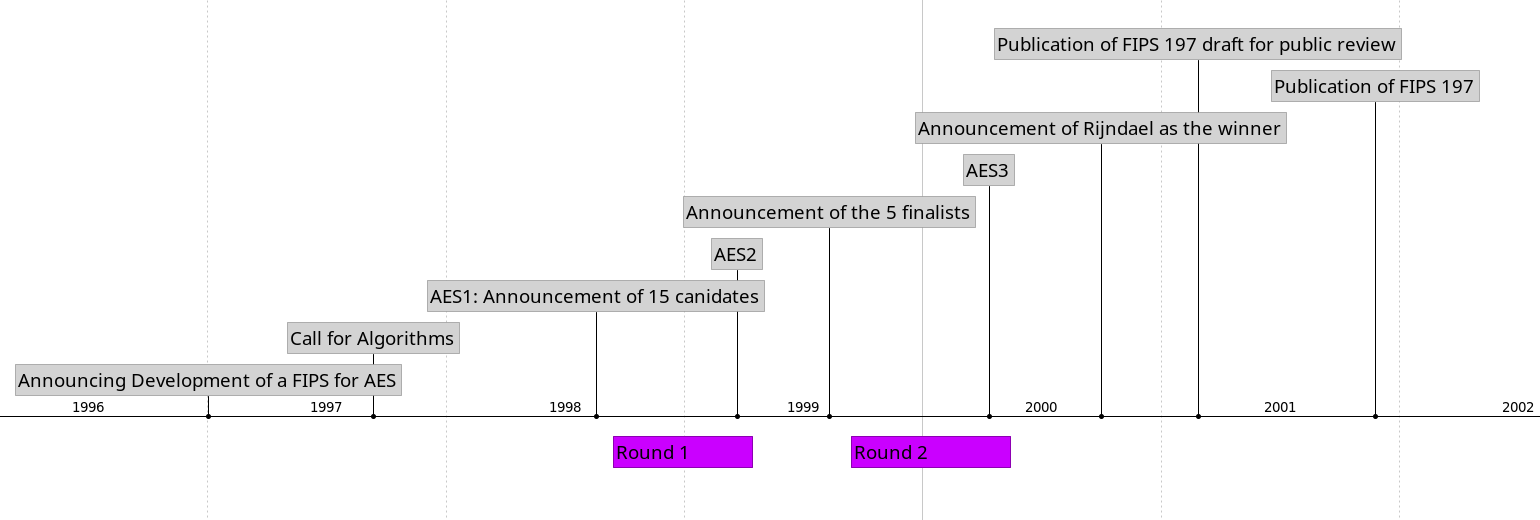
\includegraphics[scale=0.35]{aes-process-timeline.png}
\caption{AES selection process timeline}
\end{figure}

\section{AES in review}
\label{ch:aes-review}

The slightly modified Rijndael that is known as AES today has been subject to a lot of analysis over the years, with many focussing on the security aspects of the algorithm.

\subsection{NIST}
\label{ch:nist-review}

From their Round-2-Report \cite{round2report} can gain some insight in how NIST thought about Rijndael in detail. 
Although they acknowledged that some voiced critisism regarding its mathematical structure offering a potential attack vector on the algorithm, they believe that the simplicity of said structure facilitated a deeper understanding of the security properties Rijndael brings to the table. Overall they report to have no knowledge of a security attack against Rijndael.
Performance-wise they emphasise the good performance of the algorithm under a variety of circumstances, be it 8- or 64-bit software implementations, the ease, with which the algorithm is able to run in an parallel setup, the fast key setup time, low memory and disk space footprints and the speed of the hardware implementation.
NIST states that Rijndael is -thanks to its operations used- one of the easiest algorithms of the finalist to defend against power and timing sidechannel attacks. The institute did not notice a great hit in performance while testing a hardened version of Rijndael, atleast in comparison to the other finalists. Some power analysis attacks still seem to be effective though, even with the hardended Rijndael.
Key setup time and key agility were two other strong areas for Rijndael in the eyes of NIST. Furthermore the authors hint at the possibility of flexible key and block sizes, which, while not really concidered at the time of the report, is another sign in favor of Rijndael.

\subsection{Side Channel Attacks}
\label{ch:sidechannelattacks}

The cryptographer Bernstein described in \cite{bernsteincache} a successful key-extraction via network from the OpenSSL AES implementation running on a Pentium III (both very common software and hardware at the time). This sidechannel attack was in his eyes not a result of a faulty implementation, but an inherent flaw in the design of the algorithm that makes it "extremely difficult to write constant-time high-speed AES software for common general-purpose CPUs." (p.1). In many cases Bernstein can make out a correlation between the time it takes to load an array entry and the index of an entry in said array. Thus the time it takes to load an entry leaks information about the information currently processed within the algorithm ultimately revealing the key to an attacker, if said attacker can piece the leaked information together in the right way.
According to Bernstein, this is not only a problem inherent to AES, but to all cryptographic algorithm implementations that rely heavily on lookup tables to speed up their computation.
\cite{improvedcache} XXX states, that while Bernsteins "approach is widely applicable" (p.205) it critizizes this approach, because one requirement is the collection of timing data from approcimately 2^{27.5} encrypted samples. Furthermore the fragility of the Bernsteins attack is one of the main drawbacks according to te authors. The attacker needs to replicate the targeted machine with a lot of care, since small differences between target and replication will produce unusable timing data, leading to failure of the attack. Their own cache-collision timing attacks -while being orders of magnitude faster under optimal circumstances than the previously discussed attack- are representing "a significant step towards developing realistic remote timing attacks against AES" (p.210).
The power draw of the encrypting CPU seems to represent another attack vector on the algorithm. In \cite{powerdraw} the authors force the eviction of selected parts of AES lookuptables (like the SBOX) and measure the increased power draw from the CPU in case of a cache miss in the following encryption calculations. With that the authors claim to be able to extract the complete secret key. While the attack itself is descibed as "quite simple" (p.6), the same statement is made for the proposed countermeasure.
\cite{ctattacksfeasible} finds that the ease of AES-cache-behaviour exploitation is not neccessarily true anymore on more modern x86-processors. Features like multiple cores per processor with each having its own cache, the increased cache pressure emmited from more complex software, physically tagged caches, the partially undocumented and very complex prefetcher units and of course the AES-NI instruction set make it "substantially more difficult to mount data-cache side-channel attacks on AES than previously realized." (p.1). As in \cite{aes-ni} stated, AES-NI itself promises to prevent some software sidechannel attacks singlehandedly by sheer virtue of not having to use lookuptables for a fast implementation of the encryption algorithm.
This does not neccessarily apply to the slew of novel attacks categorized as 'transient execution CPU vulnerabilities' (see \cite{transientexecution}), but since they do not target AES directly they will not be discussed here.

\subsection{Mathematical Attacks}
\label{ch:mathematicalattacks}

During the AES developement the first papers with attacks on Rijndael were published. \cite{Gilbert00acollision} demonstrated an attack that broke seven rounds of AES with any key length, but the attacks "complexity is very high even if the number of plaintexts to cipher is small." (p.11). The authors did not see a danger to the complete 10-round-version.
Roughly around the same time \cite{impcryptan} published and attack, that managed to break one round more for each AES-192 and AES-256, but "[m]any of these attacks require virtually the entire codebook of texts and hence are not very practical." (p.15).
The key schedule of Rijndael was critisized in the same paper, the authors found it "worrisome" (p.15). \cite{rkeyattack} expressed similar concerns, even going as far as labeling it as weak, since it was for example enabling related-key attacks on the full rounds of AES-192 and AES-256 algorithm, which the authors found out earlier in \cite{rkeyattack2}.  While those attacks "are still mainly of theoretical interest [at the time] and do not present a threat to practical applications using AES" (p.14), or related-key attacks in general are not " not universally accepted as a practical attack model."\cite{rkeyattack3} (p.14) they also "should not be possible in a good cipher." \cite{rkeyattack} (p.13). 
\cite{rkeyattack3} continues chipping away at the confidence held in the 256-bit variant of AES, describing key derivation attacks "of practical complexity" (p.2) on a 10-round variant of that algorithm. The authors identify again the design of the key-schedule as a culprit, which they deem "not of industrial strength" (p.14). The attack seems ineffective against the 128-bit variant of the encryption algorithm. Nevertheless the authors are of the opinion, that "AES can no longer be considered as a safe black box construction, which can be dropped into any security application with little thought about how it is used."(p.14), a notion, which they think of as "disturbing"(p.14).
One of the most successful attacks on the algorithm was described in \cite{biclique} where the authors used Biclique Cryptanalysis to mount a better-than-brute-force-attack on AES with all rounds used as described in the standard, effecively reducing the key strength of each AES variant by a few bits. But even with this novel approach it still remains infeasible to recover a AES-encrypted plaintext from a ciphertext without the key or usage of side channels.


\chapter{Project Plan} \label{chap:projectplan}
% !TEX root = thesis.tex
In this chapter we will outline the project management plan from initiation to delivery. First, an overview over the different parts of the project will be given. Afterwards each phase of the project will be detailed on its own.

\section{Project Outline}
\label{ch:projectplanoutline}

The project is split into five distinct phases shown in figure \ref{fig:projectphases}. The first stage is the initiation phase outlined in \ref{ch:projectinitiation}. It contains the groundwork so the project can go ahead. No specific planning of project work is done in this phase. The second phase contains the planning of the project work and is detailed in \ref{ch:planningphase}. This includes scope management, quality management, project schedule and communications management and is the main part of the project management plan. In the execution phase described in \ref{ch:executionphase} the project work gets carried out. Progress and communications are the key aspects to manage in this phase. The fourth phase is called "Monitoring and Controlling" and describes all actions that need to take place alongside all other phases. This includes, among other things, the validation and control of the scope, quality and schedule defined in the project plan. The last phase detailed in \ref{ch:projectclosing} entails all steps that need to take place in order to deliver the final product, such as demonstration and final presentation.

\begin{figure}
  \centering
  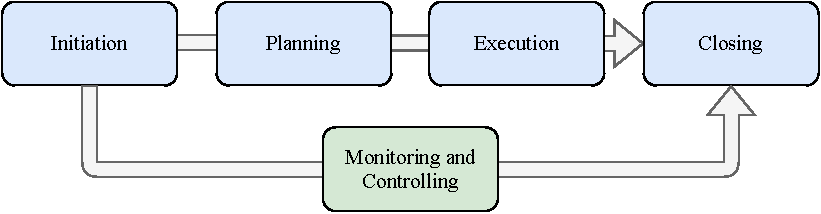
\includegraphics{data/figures/project_lifecycle.pdf}
  \caption{Project Phases}
  \label{fig:projectphases}
\end{figure}


\section{Project Initiation}
\label{ch:projectinitiation}
The project initiation is the first stage of every project. Firstly, the overall goal of the project needs to be defined on a high level. Secondly, the project manager needs to be named. In a project as small as this one, the project manager and the project team are one and the same. Thirdly, the key stakeholders are identified.


\subsection{Project Charter}
\label{ch:projectcharter}
\begin{tcolorbox}
  The overall goal of the project is a well documented implementation of the \ac{AES}. The end result should be a working piece of software that can encrypt and decrypt some input in the way defined in chapter~\ref{ch:aes}.
\end{tcolorbox}


\subsection{Project Team}
\label{ch:projectteam}
In order for the project to start the project team needs to be defined. As this project (the implementation of the \ac{AES}) will be carried out by a team of two, all team decisions have to be made at this stage. At the kick-off meeting for the project teams could be formed. After short private conversation the team for this project was decided. A meeting was setup so the first stages of planning could take place. The team for this project are Jan Phillip Berg and Simon Keil.

\subsection{Stakeholders}
\label{ch:stakeholders}
It is crucial for the project's success to identify the stakeholders and their respective interests, involvement and interdependencies. As this is a project carried out in an academic context, the stakeholders are the lecturers grading and reviewing the final work. They not only have a big impact on project success by grading the end result, but will have an involvement throughout the process with regular feedback. This feedback will be gathered through progress presentations given by the project team every two weeks. As there are no other stakeholders, the project team themselves excluded, there are no interdependencies to manage.


\section{Planning Phase}
\label{ch:planningphase}
The planning phase of the project is where the project management plan is created. This section of the thesis contains the definitions of requirements and scope, as well as the management of schedule, communications, and quality.

\subsection{Scope Management}
\label{ch:scopemanagement}
In most projects the "Magic Triangle" of scope, cost and schedule needs to be managed \cite{vanwyngaard2012}. The academic nature of this project removes considerations for cost, simplifying the planning and giving more room for playing with schedule and scope. The scope of a project should be defined as \textit{all} and \textit{only} the work required to complete the project successfully. We will define the scope of this project in the following sections by first listing the requirements. Afterwards, we will give a scope statement.

\subsubsection{Requirements}
\label{ch:requirements}
The high level goal of the project defined in chapter~\ref{ch:projectcharter} can be extended into some more detailed requirements listed below. The requirements are sorted into the those concerning the software's functionality, the implementation, and the documentation of the software.
\paragraph{Requirements on the software:}
\begin{itemize}
  \item encryption of a text input via AES-128 with a given key
  \item decryption of an encrypted text via AES-128 with a given key
  \item computation of all lookup tables used in AES-128
  \begin{itemize}
    \item computation of the SBox
    \item computation of the Round Constants for the key expansion
  \end{itemize}
\end{itemize}

\paragraph{Requirements on the implementation:}
\begin{itemize}
  \item implementation of \ac{AES} key expansion
  \item separate implementations of en- and decryption
  \item visible and even work-split between team members
  \item steady progress with biweekly presentable results
\end{itemize}

\paragraph{Requirements on the documentation:}
\begin{itemize}
  \item thesis of 20 pages containing:
  \begin{itemize}
    \item theoretical background on symmetric encryption
    \item symmetric encryption use-cases
    \item detailed explanation of the \ac{AES} algorithm
    \item project plan
    \item requirements
    \item deliverables
  \end{itemize}
  \item program documentation of 30 pages containing:
  \begin{itemize}
    \item usage
    \item implementation
    \item functions
    \item performance
    \item software stack
    \item limitations
  \end{itemize}
\end{itemize}

\subsubsection{Scope Statement}
\label{ch:scopestatement}
\begin{tcolorbox}
  The project of implementing the \ac{AES} has to goal of creating a software that can encrypt and decrypt text inputs in AES-128 with a given key. Specifically excluded from the scope are the handling of binary input, AES-256 and up, and the unification of en- and decryption functionality into one callable executable. The software only has run on one common operating system. Further compatibility is excluded from the scope. Documentation of the software and explanations of the \ac{AES}'s functionality are to be included.
\end{tcolorbox}


\subsection{Schedule Management}
\label{ch:schedulemanagement}

In order to develop a schedule the activities must be defined. We will use a work breakdown structure for this purpose, which can be found in section~\ref{ch:wbs}. Afterwards, put each \ac{WP} into a sequence and assign them to team members.

\subsubsection{Work Breakdown Structure}
\label{ch:wbs}

The work breakdown structure is shown in figure~\ref{fig:wbs}. It is a hierarchical decomposition of the work that is needed to be done in order to complete the project. The top level of this hierarchy are the five project phases detailed in section~\ref{ch:projectplanoutline}. All components of the \ac{WBS} are numbered. The lowest level component of each branch is a \ac{WP} that can be scheduled and assigned. The \ac{WBS} does not represent scheduling information. The deliverables of the project can be found in the "Execution" branch.

\begin{figure}
  \makebox[\textwidth]{
  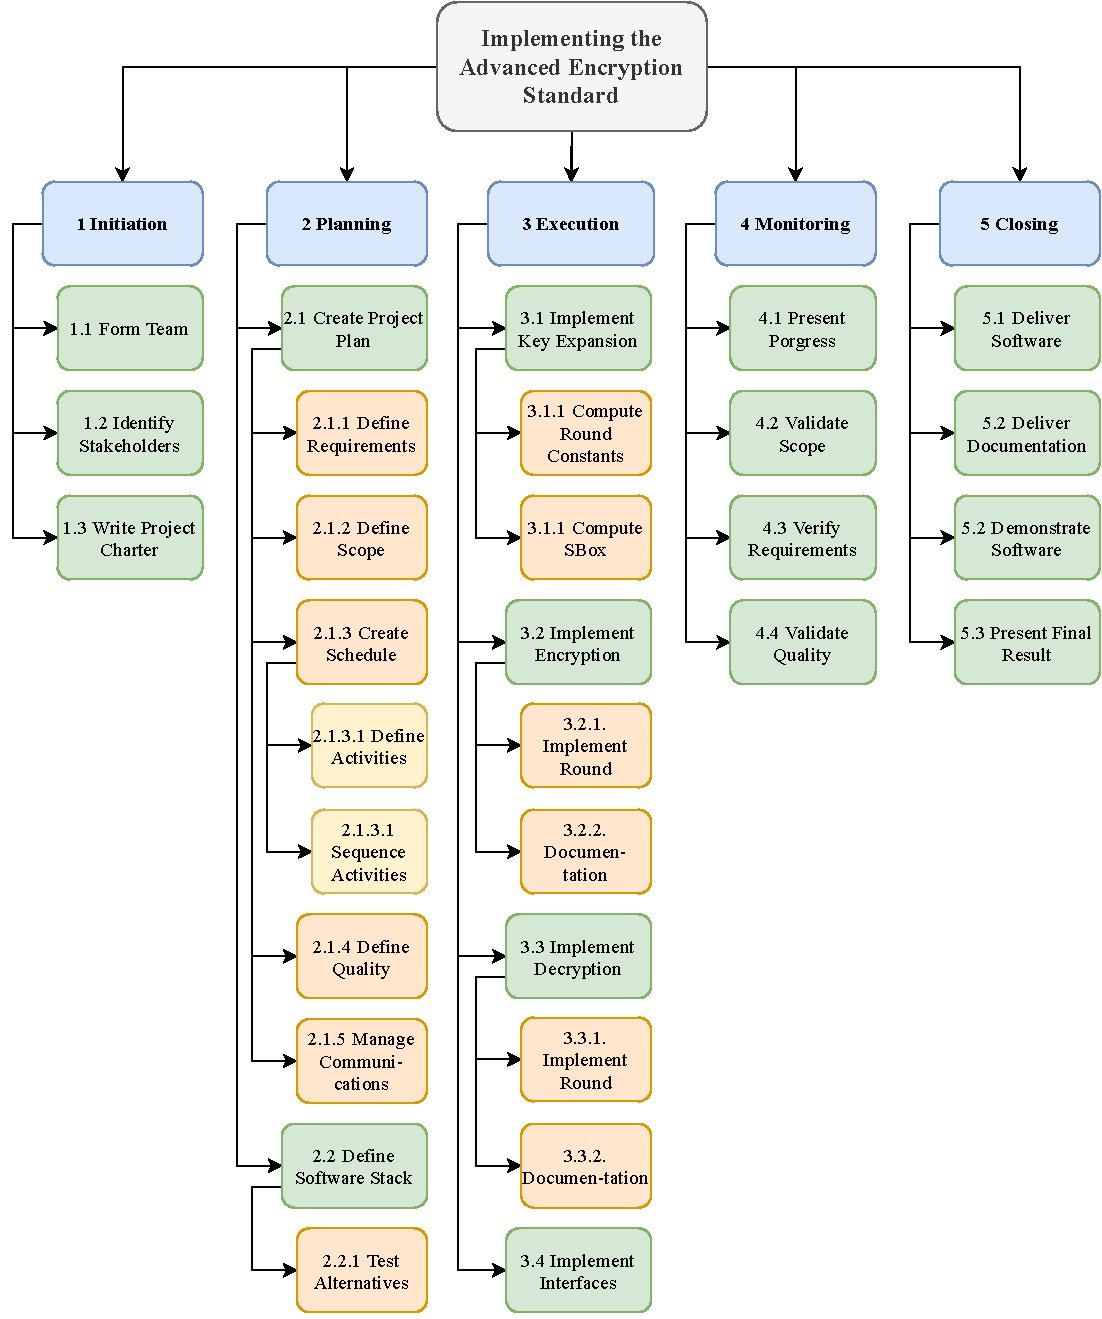
\includegraphics[scale=0.82]{data/figures/WBS.pdf}}
  \caption{Word Breakdown Structure}
  \label{fig:wbs}
\end{figure}


\subsubsection{Sequencing and Assignment of Work Packages}
\label{ch:sequencingandassignment}




\section{Quality Management}
\label{ch:qualitymanagement}
This is a software project and as such we will measure the quality of the work being done in two primary dimensions: Conformity of code to style conventions and performance or efficiency of the program. Conformity to style conventions is important in order to keep the code readable and understandable for third parties. The performance of the program has real world effects for the use of an encryption program. If the runtime is too long, encrypting large files becomes impractical.

\subsection{Code Quality}
\label{ch:codequality}
For Python code we will refer to the PEP-8 style guide \cite{pep8}. Code files will be organized by logical program parts. For C Code we will refer to the .... style guide. We will include C source files as well as header files in the code directories. Functions should have docstrings. Where inline comments are necessary to explain actions, their use is encouraged. In general, the use of inline comments should be minimal.

\subsection{Program performance}
\label{ch:programperformance}
Program performance highly depends on the time complexity of the algorithms, the inputs to the program, as well as the software stack that is used. As the algorithm and the inputs are given for this project, the software stack is the major contributing factor to program performance. In general, the lower level a language is, the faster you can make a program. Writing the software in assembly or even a hardware description language to program a \ac{FPGA} would yield the best results. However, we deem these options to be out of scope for this project. Which software stack was chosen and why is detailed in section~\ref{ch:softwarestack}.

To measure the performance of our implementation, reference implementations in various higher level languages are given the same inputs. We then compare the results with our solution. For the different subparts of the program, different implementations of single functions are to be tested against each other to find the best compromise between performance and code quality. An example of this would be converting string inputs into bytes through string operations versus through bit-shifts.

The quality goal for performance is an implementation that is faster than implementations in pure Python.

DIFFERENT TIMINGS HERE

\subsection{Software Stack}
\label{ch:softwarestack}
The selection of the software stack depends on a few major factors. Those factors are the platform the program should run on, developer experience, and performance. The stack that was chosen for this project is shown in figure~\ref{fig:stack}

In the team formation process discussed in section~\ref{ch:projectteam} the literacy in various programming languages was a key component. We decided on Python 3 as our wrapper language. This means all one-time operations will be written in Python. This makes the code readable without incurring major performance penalties. Another advantage of using Python is that the software will run on most platforms. Both team members are fluent and have experience writing code in Python.

The performance goals defined in section~\ref{ch:programperformance} are not reachable with pure Python. Therefore, we select to write the core algorithms in C. The main benefit of this hybrid approach is performance. The disadvantage is the increased code complexity inherent to C. The approach also requires an interface between C and Python.

After testing different interface solutions we settled on the ctypes module for Python 3 \cite{ctypes}. The major advantage is that we can write normal independent C code and compile it separately. Other solutions would have required non-standard interpreters or compilers (see Cython \cite{cython}). The interface works by compiling the C code into libraries and importing those into a Python program. The functions within are then callable in Python. Intercompatibility between platforms is maintained by shipping with C source and header files. Compilation can be done according to the platform.

\begin{figure}
  \centering
  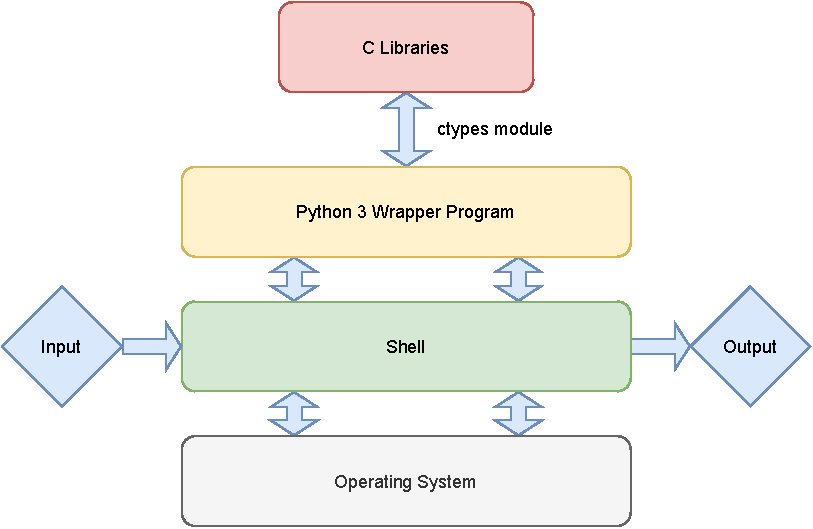
\includegraphics{data/figures/stack.pdf}
  \caption{Software Stack}
  \label{fig:projectphases}
\end{figure}


\subsection{Communications Management}
\label{ch:communicationsmanagement}
Communication is a key part of every project. Even though the team for this project only has two members communication channels need to be well defined. In software project such as this one the source code management is also a concern. Another key component of the communications management is the engagement with the projects stakeholders. The communication channels for all these purposes are detailed below.

\subsubsection{Source Code Management and Version Control}
\label{ch:versioncontrol}
The version control tool of choice is Git \cite{git}. A remote repository will be hosted on \url{github.com}. We follow a loose feature-branch workflow. Separate branches are created for the key components (work packages 3.1, 3.2, 3.4 see~\ref{ch:wbs}) of the software, as well as for the documentation and thesis documents. Team members work on the branches of the work packages they are assigned to (see ~\ref{ch:sequencingandassignment}). Merging into other branches occurs when the component is complete. Testing is done on each component separately before merging.


\subsubsection{Day to Day Communications}
\label{ch:daytodaycomms}
For day to day issues a WhatsApp chat is used as the primary communications channel. It ensures high availability. Reasons to use this channel might be: arranging of code interfaces, scheduling of meetings, and questions or problems regarding project. Progress is discussed in regular meetings via Zoom. These meetings are scheduled at least weekly.


\subsubsection{Stakeholder Engagement}
\label{ch:stakeholerengagement}
As discussed in section~\ref{ch:stakeholders}, the main stakeholders for this project are the lecturers grading the final work. They are engaged in the process through biweekly presentations of the progress. These presentations are around ten minutes in length and entail both team members discussing their progress during the time in between sessions. Both team members need to present their respective work and demonstrate the even split of workload during the whole project. Stakeholder engagement is important in order to keep on track and avoid scope- or schedule creep.


\section{Execution Phase}
\label{ch:executionphase}
The execution phase is the main part of the project. The team members work on their assigned \ac{WP}s and create the deliverables for the project. All parts of the project done in this phase can be found in execution branch of the \ac{WBS}. While implementation and documentation takes place, the communication needs to be managed according to the communications management plan laid out in section~\ref{ch:communicationsmanagement}. Regular meetings between team members take place to discuss progress and problems that might have arisen. Progress presentations to the stakeholders happen biweekly. In addition to the main tasks, these presentations need to be prepared. This is an important step in order for the team to mark the progress.

While the main \ac{WP}s get worked on, the monitoring and controlling processes detailed in section~\ref{ch:monitoringcontrolling} need to be carried out alongside. This mainly includes the testing of implemented functionality. Rigorous testing and validation ensures the final software is inside the defined quality and scope. Readjustments to scope and requirements need to be made whenever there is new input from the stakeholders or the current scope or requirements are not achievable any more. Regular reassessment and verification is crucial to project success.


\section{Monitoring and Controlling}
\label{ch:monitoringcontrolling}
This section details the processes that take place alongside the main schedule. They serve the purpose to keep the project on track, meaning in scope, in quality, and on schedule. Without these processes project success is much harder to achieve. As these monitoring and controlling functions are regular tasks each team member needs to do they are listed in the \ac{WBS}. In the following, these processes are described in further detail.

\subsection{Validate Scope}
\label{ch:validatescope}
Every time a \ac{WP} is completed, the project team will validate that the deliverable is inside project scope. If it is not sufficient, a change request will be made to the assigned team member. They will start implementing the changes decided on. This workflow ensures all deliverables meet the requirements and that the project is in scope.

In regular intervals the project team will reassess whether the scope statement (see section~\ref{ch:scopestatement}) is still accurate. The project scope will be adjusted if stakeholders demand changes or if the schedule cannot be met. Such changes need to be decided on with the whole project team. They need to be formalized in a new scope statement and changes to the \ac{WBS} and schedule need to be made accordingly. This formalization of changes is important to ensure all team members are on the same page regarding the scope of the project.

\subsection{Verify Requirements}
\label{ch:verifyrequirements}
In accordance with the workflow laid out in section~\ref{ch:validatescope}, finished \ac{WP}s need to be assessed against the project requirements. If the deliverable is lacking, change requests are implemented. Alongside the verification of requirements for each \ac{WP}, the project requirements need to be reevaluated analogous to scope reassessment. New requirements can only be added if formalized. Sources of changes to the requirements are schedule conflicts and stakeholder requests.

\subsection{Validate Quality}
\label{ch:validatequality}
Each function in the program code needs to be validated on its quality. The guidelines for quality can be found in section~\ref{ch:qualitymanagement}. In regular progress meetings the team members talk each other through all \ac{WP}s they are working on (finish as well as in progress). Assessments regarding code quality and conformity to style conventions can be made in these meetings. Checking for style conventions will also be automated in the Git repository.

Each team member is responsible for testing their code throughout the process. Bugs are to be fixed in order to maintain a working program. When user input is taken, it needs to be properly escaped. Testing for edge-cases needs to be done. Testing for program performance will at the delivery of each larger component (\ac{WP} 3.1, 3.2, 3.3, 3.4). If performance is lacking, the team member assigned to that component needs to optimize the code. Solutions for optimization problems can be found in weekly meetings.

\subsection{Present Progress}
\label{ch:presentprogress}
As detailed in section~\ref{ch:stakeholerengagement}, biweekly progress presentations will take place during the project duration. In these presentations each project team member will present what they have accomplished over the last two weeks. This monitoring process is important in order to keep the work going at a steady rate and ensure an equal work split between team members. These presentations are as much for the stakeholders as they are for the project team. The regularity of presentations keeps the team schedule by having external deadlines.


\section{Project Closing and Delivery}
\label{ch:projectclosing}
When all project work is done, all deliverables will be combined into one release. The release will contain the final software as defined by the scope statement in section~\ref{ch:scopestatement}. Alongside the software the final delivery will include the thesis and program documentation as mentioned in section~\ref{ch:requirements}. Before delivering, the project team will run through the monitoring processes again to ensure the final delivery is in scope and up to the defined quality standards. The last progress presentations will be a demonstration of the final software as well as short presentation of all its source code. This presentation constitutes the delivery of the final product.

After the conclusion of the project, a reflection phase might occur. The team will meet to discuss what did and what did not go to plan in order to learn from shortcomings.


%% include appendix
\appendix
%!TEX root = thesis.tex
%This is only relevant for TeXShop
\chapter{Appendix A}
\label{ch:appendixa}

\begin{figure}[h]
\centering
\includegraphics[width=\textwidth]{data/figures/aes.png}
\caption{The unencrypted bitmap-file converted to a .png-file.}
\label{fig:aespng}
\end{figure}

\begin{figure}[h]
\centering
\includegraphics[width=\textwidth]{data/figures/aesECB.png}
\caption{The bitmap-file encrypted with AES in ECB mode and converted to a .png-file. The writing "Advanced Encryption Standard" is clearly readable, despite the encryption.}
\label{fig:aesecbpng}
\end{figure}

\begin{figure}[h]
\centering
\includegraphics[width=\textwidth]{data/figures/aesCTR.png}
\caption{The bitmap-file, encrypted with AES in CTR mode and converted to a .png-file. To the naked eye the content of the picture is indistinguishable from noise.}
\label{fig:aesctrpng}
\end{figure}


\begin{table}[h]
  \resizebox{\textwidth}{!}{%
  \begin{tabular}{c | c c c c c c c c c c c c c c c c c}
    & 0 & 1 & 2 & 3 & 4 & 5 & 6 & 7 & 8 & 9 & a & b & c & d & e & f \\ \hline
    0 & 0x63 & 0x7c & 0x77 & 0x7b & 0xf2 & 0x6b & 0x6f & 0xc5 & 0x30 & 0x01 & 0x67 & 0x2b & 0xfe & 0xd7 & 0xab & 0x76 \\  1 &  0xca & 0x82 & 0xc9 & 0x7d & 0xfa & 0x59 & 0x47 & 0xf0 & 0xad & 0xd4 & 0xa2 & 0xaf & 0x9c & 0xa4 & 0x72 & 0xc0 \\ 2 &  0xb7 & 0xfd & 0x93 & 0x26 & 0x36 & 0x3f & 0xf7 & 0xcc & 0x34 & 0xa5 & 0xe5 & 0xf1 & 0x71 & 0xd8 & 0x31 & 0x15 \\ 3 & 0x04 & 0xc7 & 0x23 & 0xc3 & 0x18 & 0x96 & 0x05 & 0x9a & 0x07 & 0x12 & 0x80 & 0xe2 & 0xeb & 0x27 & 0xb2 & 0x75 \\ 4 & 0x09 & 0x83 & 0x2c & 0x1a & 0x1b & 0x6e & 0x5a & 0xa0 & 0x52 & 0x3b & 0xd6 & 0xb3 & 0x29 & 0xe3 & 0x2f & 0x84 \\ 5 & 0x53 & 0xd1 & 0x00 & 0xed & 0x20 & 0xfc & 0xb1 & 0x5b & 0x6a & 0xcb & 0xbe & 0x39 & 0x4a & 0x4c & 0x58 & 0xcf \\ 6 & 0xd0 & 0xef & 0xaa & 0xfb & 0x43 & 0x4d & 0x33 & 0x85 & 0x45 & 0xf9 & 0x02 & 0x7f & 0x50 & 0x3c & 0x9f & 0xa8 \\ 7 & 0x51 & 0xa3 & 0x40 & 0x8f & 0x92 & 0x9d & 0x38 & 0xf5 & 0xbc & 0xb6 & 0xda & 0x21 & 0x10 & 0xff & 0xf3 & 0xd2 \\ 8 & 0xcd & 0x0c & 0x13 & 0xec & 0x5f & 0x97 & 0x44 & 0x17 & 0xc4 & 0xa7 & 0x7e & 0x3d & 0x64 & 0x5d & 0x19 & 0x73 \\ 9 & 0x60 & 0x81 & 0x4f & 0xdc & 0x22 & 0x2a & 0x90 & 0x88 & 0x46 & 0xee & 0xb8 & 0x14 & 0xde & 0x5e & 0x0b & 0xdb \\ a & 0xe0 & 0x32 & 0x3a & 0x0a & 0x49 & 0x06 & 0x24 & 0x5c & 0xc2 & 0xd3 & 0xac & 0x62 & 0x91 & 0x95 & 0xe4 & 0x79 \\ b & 0xe7 & 0xc8 & 0x37 & 0x6d & 0x8d & 0xd5 & 0x4e & 0xa9 & 0x6c & 0x56 & 0xf4 & 0xea & 0x65 & 0x7a & 0xae & 0x08 \\ c & 0xba & 0x78 & 0x25 & 0x2e & 0x1c & 0xa6 & 0xb4 & 0xc6 & 0xe8 & 0xdd & 0x74 & 0x1f & 0x4b & 0xbd & 0x8b & 0x8a \\ d & 0x70 & 0x3e & 0xb5 & 0x66 & 0x48 & 0x03 & 0xf6 & 0x0e & 0x61 & 0x35 & 0x57 & 0xb9 & 0x86 & 0xc1 & 0x1d & 0x9e \\ e & 0xe1 & 0xf8 & 0x98 & 0x11 & 0x69 & 0xd9 & 0x8e & 0x94 & 0x9b & 0x1e & 0x87 & 0xe9 & 0xce & 0x55 & 0x28 & 0xdf \\ f & 0x8c & 0xa1 & 0x89 & 0x0d & 0xbf & 0xe6 & 0x42 & 0x68 & 0x41 & 0x99 & 0x2d & 0x0f & 0xb0 & 0x54 & 0xbb & 0x16 \\
  \end{tabular}
  }
  \caption{Sbox}
  \label{sbox}
\end{table}


\chapter{Acronyms}
% !TEX root = thesis.tex
% List of acronyms
%-- \ac{betai} f�gt die Abk�rzung ein. Beim ersten Vorkommen der Abk�rzung wird zun�chst der ganze Begriff angegeben und das Akronym bzw. die Abk�rzung in Klammern.
%-- \acs{betai} wird dann nur das Symbol bzw. die Abk�rzung im Text gedruckt
%-- \acf{betai} gibt zus�tzlich noch die Erkl�rung aus
%-- \acl{betai} f�gt lediglich die Beschreibung ein.
%\chapter{Acronyms}
\begin{acronym}
 \setlength{\itemsep}{0.2em}
 \acro{BPMN}{business process model and notation}
 \acro{FFT}{fast Fourier transformation}
 \acro{IMEI}{international mobile station equipment identity}
 \acro{MAC}{media access control}
 \acro{MEMS}{microelectromechanical system}
 \acro{PCA}{principal component analysis}
 \acro{RSS}{root sum square}
 \acro{UDID}{unique device identifier}
 % etc.
 \acro{AES}{Advanced Encryption Standard}
 \acro{WBS}{work breakdown structure}
 \acro{FPGA}{Field Programmable Gate Array}
 \acro{WP}{Work Packages}
\end{acronym}
 % optional, remove it if you do not like it

\pagestyle{scrplain} % turn off headers and footers
% generate list of figures, optional, remove it if you do not like it
\listoffigures
\cleardoublepage

% generate list of tables, optional, remove it if you do not like it
\listoftables
\cleardoublepage

% generate list of algorithms, optional, remove it if you do not like it
\phantomsection
\addcontentsline{toc}{chapter}{List of Algorithms}
\listofalgorithmes
\cleardoublepage

% generate list of listings, optional, remove it if you do not like it
\renewcommand*{\lstlistlistingname}{List of Listings}
\lstlistoflistings
\cleardoublepage

% generate bibliography with bibtex, the bibfile here is "paper.bib"
% use alphanumerical style
\flushbottom
\bibliography{references}

% legal declarations
\cleardoublepage
\declarationofauthorship{\thesislanguage}{\thesistitle}
\cleardoublepage
\consentforplagiarismdetection{\thesislanguage}{\authorname}{\studentnumber}{\courseofstudy}{\thesistitle}

% do not forget to add a CD/DVD with the digital version of your thesis (pdf and LaTeX) as well as the source code of your project

\end{document}
